%%%---------------------------------------------------------------%%%
%%% Wyzsza Szkola Gospodarki Bachelor's Thesis                    %%%
%%% Prepared by Bruno Axel Kamere                                 %%%
%%% Inspired by Artur M. Brodzki & Piotr Woźniak's WUT template.  %%%
%%% Computer Engineering and Mechatronics Department              %%%
%%% Wyzsza Szkola Gospodarki w Bydgoszczy, 2022                   %%%
%%%---------------------------------------------------------------%%%
% -------------------------------------------------------------------
% 30. Methodology and setup                                         %
% -------------------------------------------------------------------


%/-------------------------------- CHAPTER START --------------------------------/%

\chapter{Methodology and setup}
\label{chap:methodology-and-setup}

In this chapter, the solution is going to be explained in details. The reason behind various design choices is going to be explained elaborately as well as the technical aspects of the solution.

%/-------------------------------- SECTION START --------------------------------/%

\section{Approach}
\label{sec:approach}

In the early stages of the development, the main idea was that the solution had to be:

\begin{itemize}
    \item Well planned. Every step taken had to be thought of, usually drawn on a paper to assess its feasibility. Figure \ref{fig:initial-draft-designs} shows the initial draft designs during the brainstorming phase of the solution development.
    \item Well-built. The project had to be well-structured such that it is intuitive to navigate around source codes. A specific naming convention was followed throughout the source codes to maintain a consistent code base.
    \item Easily maintainable. The project was broken down into segments of folders with inheritance.
    \item Built with professional, software engineering industry toolset, as described in section \ref{sec:tools-used}.
    \item Agile. The AWS infrastructure mainly had to be built such that it is easy to deploy and destroy without investing a lot of effort.
\end{itemize}

With the above points in mind, the solution design process started on paper. Figure \ref{fig:initial-draft-designs} shows some initial designs of the proposed system. After several design iterations, final designs were produced like the AWS architecture high-level design in figure \ref{fig:aws-architecture-hld}. The next step was then to bring the designs to reality. And that was no easy task.

\begin{figure}[H]
    \centering 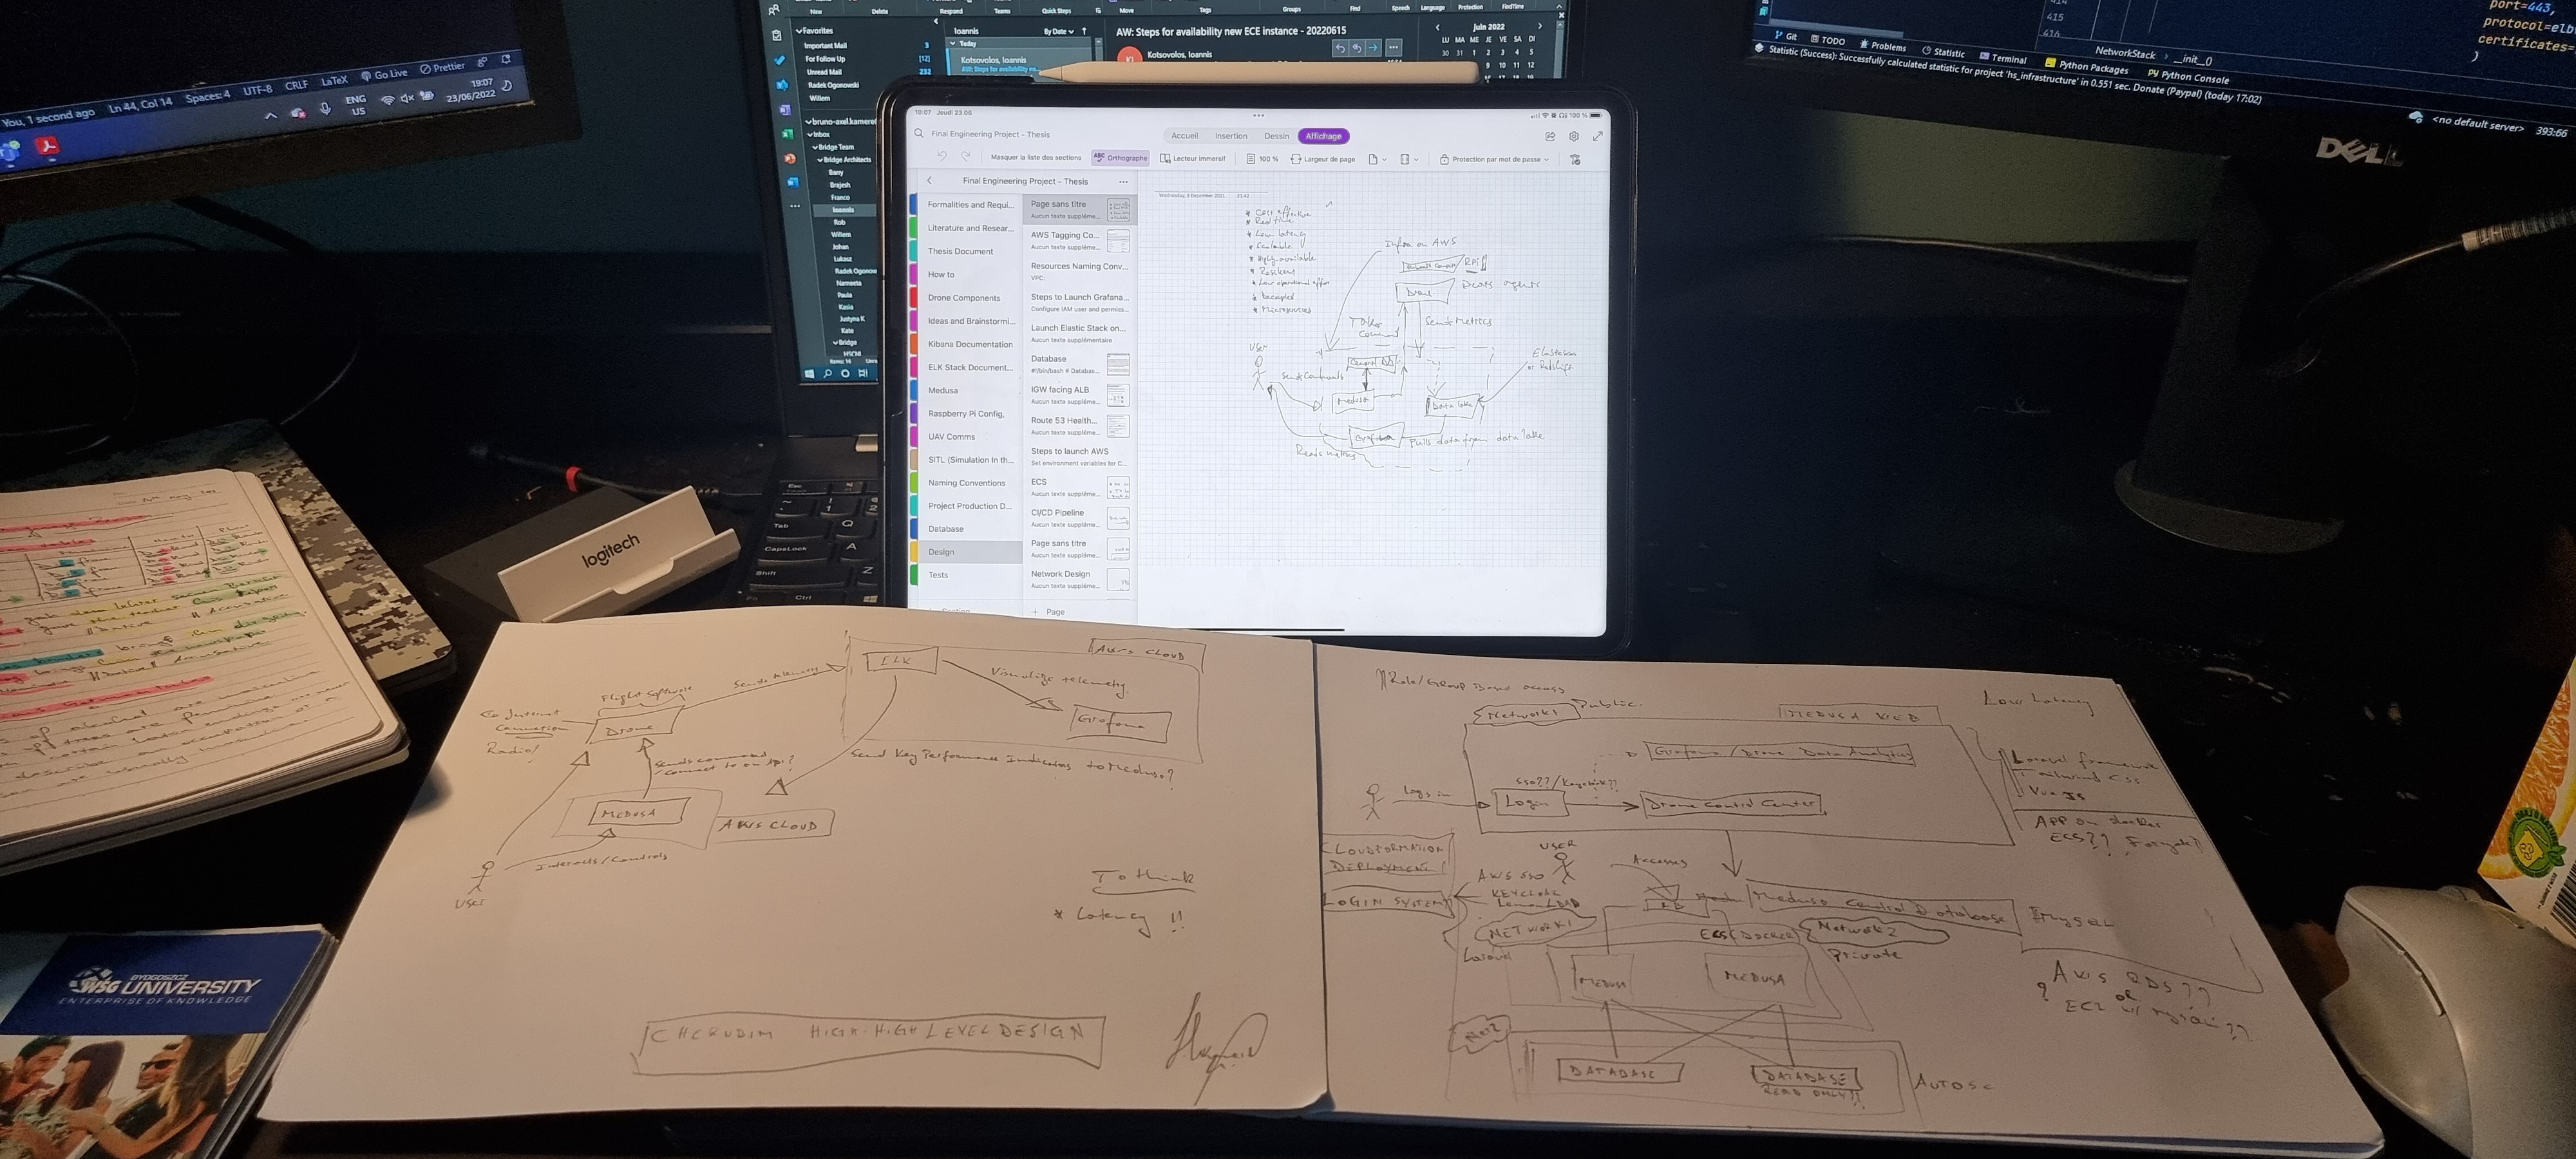
\includegraphics[width=1\linewidth]{initial_designs_2.jpg}
    \caption{Initial draft architecture designs.}
    \label{fig:initial-draft-designs}
    \source{Own work.}
\end{figure}

As the design started being built to reality, it was evident that deploying the whole AWS infrastructure manually from the AWS console, see figure \ref{fig:aws-console-home}, was going to be a time-consuming and inefficient activity. And this also contradicted the initial idea of building an agile infrastructure that can be easily redeployed in case changes are needed. That is where the thought to build the infrastructure as code using some sort of infrastructure as code (IaC) tool came in. Since the cloud provider of choice was AWS, the best tool for the task was with no doubt the AWS' very own cloud development kit\cite{awscdkdocumentation}.

After the AWS infrastructure was built, the next step was the UAV. The outstanding questions here were:

\begin{itemize}
    \item How is the UAV going to be built?
    \item What is going to be the size?
    \item What is going to be the UAV type? Quadcopter? Fixed wing?
    \item How is the UAV going to be programmed? What programming language should be used?
    \item How is the UAV going to communicate with the rest of the system on AWS?
\end{itemize}

The above questions drove the next development stage. The UAV type of choice was a small quadcopter. The initial idea was to build an actual quadcopter, therefore the below parts were purchased to build the quadcopter from scratch, figure \ref{fig:quadcopter-hardware-components} shows the components:

\begin{itemize}
    \item ReadytoSky S500 quadcopter frame with built-in PCB.
    \item Pixhawk 2.4.8 flight controller with 4 GB of onboard SD card storage.
    \item Raspberry Pi 4 model B with 4 GB of onboard SD card storage.
    \item ReadytoSky M8N GPS module built-in compass with GPS antenna mount.
    \item 4 pieces of A2212 1000KV brushless motors.
    \item 4 pieces of 2-6S 30 amps Electronic speed controllers.
    \item 2 pairs of 1238 carbon fibre propellers.
\end{itemize}

\begin{figure}[H]
    \centering \includegraphics[width=1\linewidth]{quadcopter_components_compressed.png}
    \caption{Quadcopter hardware components.}
    \label{fig:quadcopter-hardware-components}
    \source{Own work.}
\end{figure}

As the development of the quadcopter went on, it became obvious that this approach was not the best way to go, especially for a proof-of-concept (POC) solution mainly due to how costly it was becoming. At some point the wire connectors were even insufficient, and it came to notice that a power module was also needed, and it would take too long to order the parts online. The idea to build the actual physical quadcopter was then put on-hold, and it was decided to rather use simulation tools to simulate the actual quadcopter. Section \ref{sec:software-in-the-loop} elaborates more on how the simulation was implemented and set up.

%/--------------------------------- SECTION END ---------------------------------/%


%/-------------------------------- SECTION START --------------------------------/%

\section{Solution description}
\label{solution-description}

The proposed solution is a bit vast, here below the designs are going to be described and explained.

%/------------------------------ SUB-SECTION START ------------------------------/%

\subsection{AWS architecture high-level design}
\label{subsec:aws-architecture-hld}

One of the solution development best practice is to design first before attempting implementation. This helps one to brainstorm beforehand how the solution to be built will look like. This approach was followed in developing the proposed solution. Figure \ref{fig:aws-architecture-hld} shows the high-level design that pictures a holistic view of how the AWS infrastructure looks like. It pictures how various AWS services talk to each other and how. The design is labelled with numbers, which are used to explain what each link is for in the following paragraph. Some components shown in design were not fully implemented but are part of the design as future work, that includes the continuous integration and continuous delivery (CI/CD) pipeline section on the left of the design, though it was tested separately and proven to work.

\begin{figure}[H]
    \centering 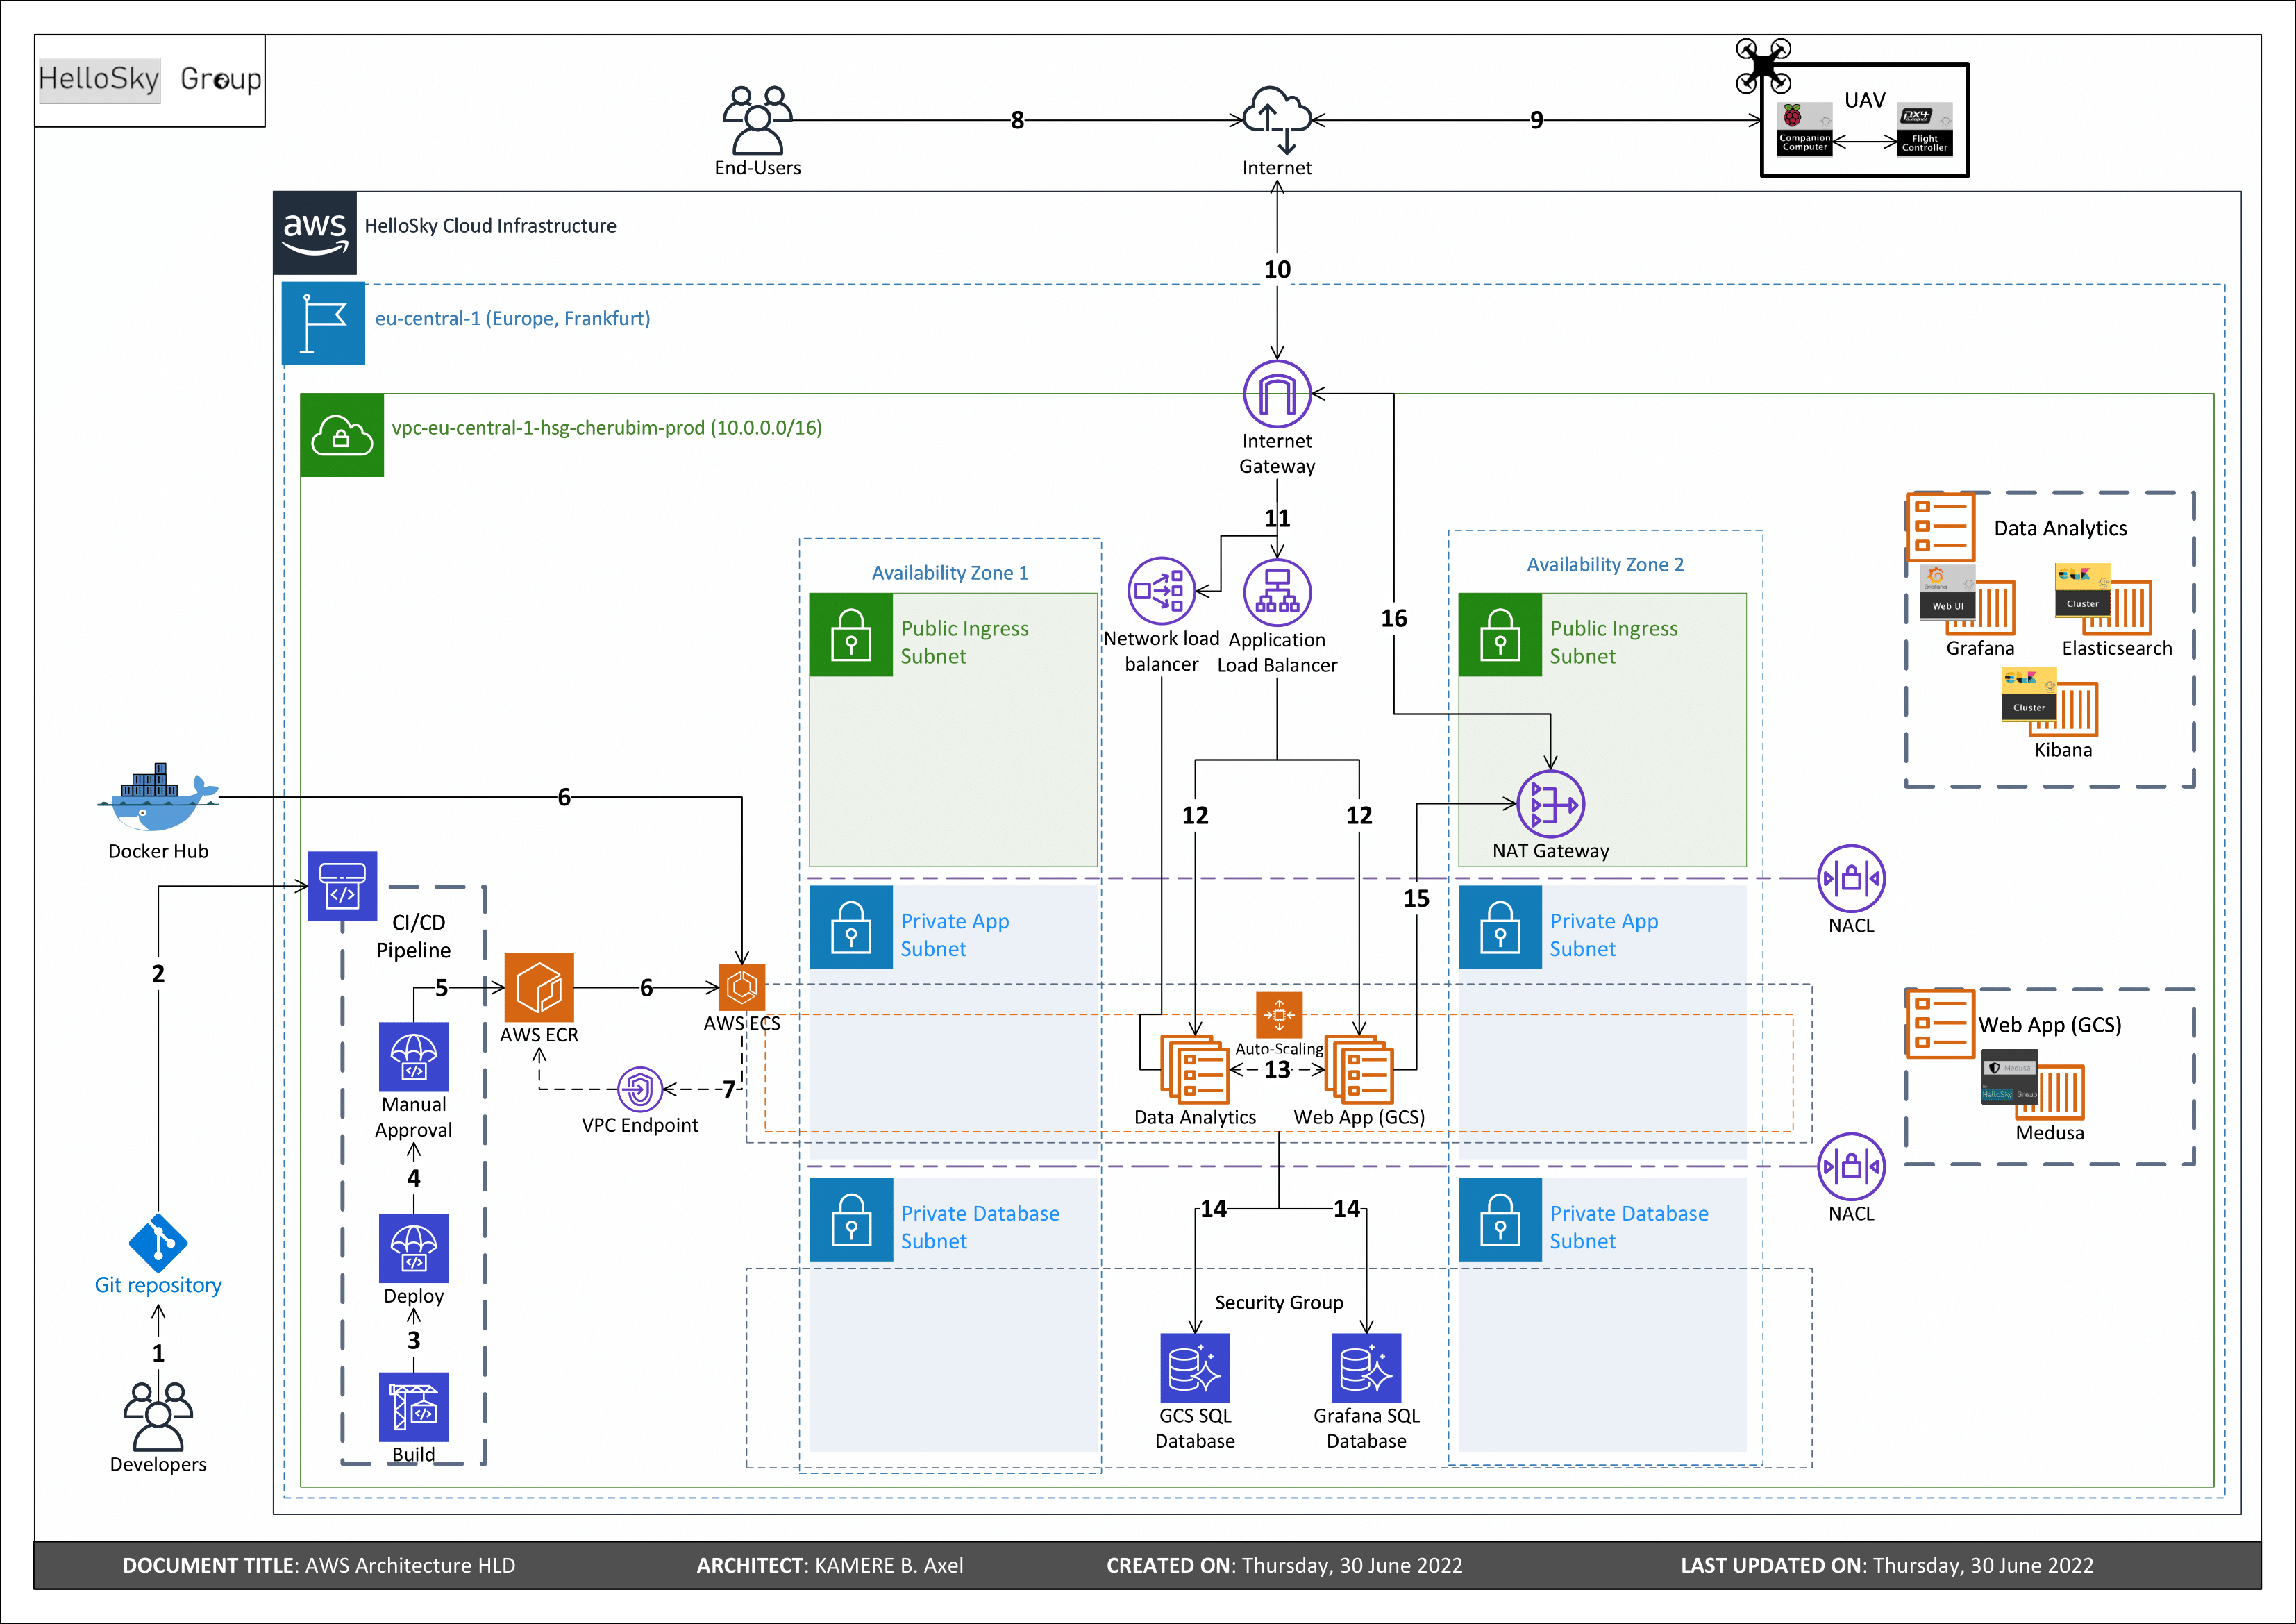
\includegraphics[width=1\linewidth]{aws_architecture_hld.png}
    \caption{Proposed AWS architecture high-level design.}
    \label{fig:aws-architecture-hld}
    \source{Own work. Designed with Microsoft Visio. Refer to \ref{subsec:ms-visio}.}
\end{figure}

Below are the explanations of the numbered items in the figure \ref{fig:aws-architecture-hld}:

Number 1 through 5 is a CI/CD pipeline that builds a docker image of the web app, the ground control station deployed on cloud.

\begin{enumerate}
    \item Developers commit code changes to a master branch of a Git repository.
    \item The activity triggers an AWS CloudWatch alarm, which then initiates the AWS CodePipeline.
    \item AWS CodeBuild service compiles the source code, runs tests and returns packaged application images ready to be deployed.
    \item After a package is created, the pipeline now waits for manual approval by an approver. This is so that only approved code are deployed to a production environment.
    \item Approved packaged images are pushed to the AWS Elastic Container Registry (ECR).
    \item Packages are pulled either from Docker Hub registry or from AWS ECR to build AWS containerized services.
    \item AWS Elastic Container Service (ECS) pulls images from AWS ECR via an AWS Virtual Private Cloud endpoint (VPC endpoint).
    \item Users can access front-end applications deployed on AWS through the internet
    \item The UAV sends telemetry to AWS services like the data lake and ground control station (GCS) and receives mission commands from the GCS via an LTE or Wi-Fi data link.
    \item All traffic that go to an AWS VPC have to go through an internet gateway. Without it, AWS VPC resources cannot talk to the internet.
    \item All incoming traffic is load balanced with an AWS application load balancer (AWS ALB) which will then forward the traffic to desired services depending on the requested resource.
    \item Traffic is routed to the desired target group configured on the AWS ALB.
    \item The GCS and data analytics services like the telemetry dashboards and the data lake can communicate to each other.
    \item Grafana that runs the telemetry dashboards has a MySQL database that the Grafana service can access in the private isolated subnet. The same goes for the GCS.
    \item Resources deployed in private have no direct communication with the internet, therefore for them to pull updates, a network address translation gateway (NAT gateway) is needed to establish the connection.
    \item The NAT gateway the goes through the internet gateway then to the internet.
\end{enumerate}

%/------------------------------- SUB-SECTION END -------------------------------/%


%/------------------------------ SUB-SECTION START ------------------------------/%

\subsection{AWS cloud development kit setup}
\label{subsec:aws-cdk-setup}

The AWS infrastructure described in section \ref{subsec:aws-architecture-hld} is deployed as code using AWS cloud development kit (AWS CDK). AWS CDK allows developers to build AWS infrastructures in an agile manner by using normal programming languages. This allows developers to take advantage of programming idioms like loops, variables, conditionals and inheritance to build robust AWS infrastructures. This also means that software engineering practices like source control, testing and code reviews can be used since the infrastructure is basically standard code. Currently, AWS CDK supports Python, JavaScript, C\#, Go, and Typescript programming languages.

A typical AWS CDK project is made up of 3 components, namely:

\begin{itemize}
    \item An app. This is the overall set of everything. An AWS CDK project is basically called an AWS CDK app. This consists of constructs.
    \item Constructs. These represent components that make an AWS infrastructure. They can be an AWS simple storage service (S3), an elastic cloud compute (EC2), an application load balancer (ALB) \textit{et cetera}. AWS has a comprehensive site that shows all the available AWS and community constructs\cite{awsconstructhub}.
    \item Stacks. These are the unit of deployment in AWS CDK. A stack represents all AWS resources defined within the same scope.
\end{itemize}

Figure \ref{fig:aws-cdk-app-structure} shows how an AWS CDK app is structured.

\begin{figure}[H]
    \centering 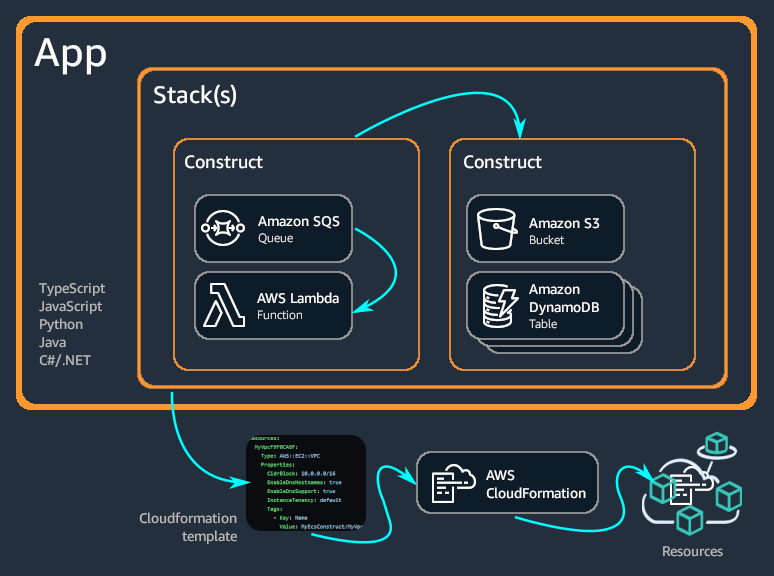
\includegraphics[width=1\linewidth]{aws_cdk_workflow.png}
    \caption{AWS CDK app structure.}
    \label{fig:aws-cdk-app-structure}
    \source{AWS CDK documentation\cite{awscdkdocumentation}.}
\end{figure}

%/------------------------------- SUB-SECTION END -------------------------------/%


%/------------------------------ SUB-SECTION START ------------------------------/%

\subsection*{Build}
\label{subsec:build}

To start building the AWS infrastructure with AWS CDK, the AWS command line interface (CLI) needs to first be set up. To install the AWS CLI on Windows, run the following command \mintinline[breaklines, breakanywhere]{bash}{msiexec.exe /i https://awscli.amazonaws.com/AWSCLIV2.msi}. This allows to interact with AWS via the CLI.

Once the AWS CLI is installed, type the command \mintinline[breaklines, breakanywhere]{bash}{aws configure} to configure credentials to AWS. The console will ask for the AWS access key ID, the AWS secret access key, the default region name and the default output format as shown in figure \ref{fig:aws-configure-output}.

\begin{figure}[H]
    \centering 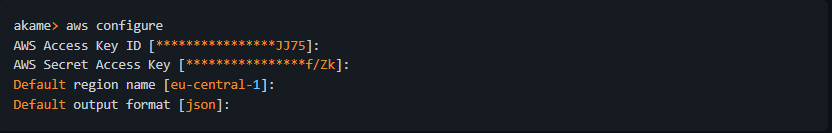
\includegraphics[width=1\linewidth]{aws_configure_output.png}
    \caption{AWS configure CLI output.}
    \label{fig:aws-configure-output}
    \source{Own work.}
\end{figure}

The next step is to then install AWS CDK from node package manager (NPM) with \mintinline[breaklines, breakanywhere]{bash}{npm install -g aws-cdk}. This will download and install the latest aws-cdk package on the local workstation. The '-g' flag makes the package available globally on the workstation.

Next, get the account number from the AWS CLI using the AWS security token service (STS) and the region name from AWS CLI configuration by executing the commands below.

\mintinline[breaklines, breakanywhere]{bash}{aws sts get-caller-identity}, to get the account number.

\mintinline[breaklines, breakanywhere]{bash}{aws configure get region}, to get the region name.

\begin{figure}[H]
    \centering 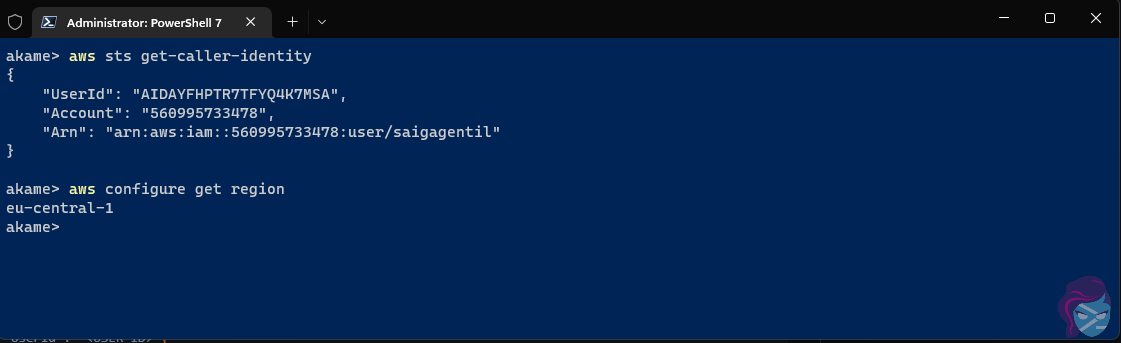
\includegraphics[width=1\linewidth]{cdk_pre_bootstrap.png}
    \caption{AWS STS and configure commands output.}
    \label{fig:aws-account-numbre-region}
    \source{Own work.}
\end{figure}

With the account number and the region name, AWS CDK can be bootstrapped now. Bootstrapping in AWS refers to the process of creating assets (local files, directories, docker image, \textit{et cetera}) that need to be deployed with the stack. These assets are deployed to an AWS S3 bucket for AWS CloudFormation to use them during stack deployment. Execute command \mintinline[breaklines, breakanywhere]{bash}{cdk bootstrap aws://560995733478/eu-central-1} to bootstrap AWS CDK.

Once all the above steps are completed, a CDK app can now be created. First create a directory for the app and move into the directory, \mintinline[breaklines, breakanywhere]{bash}{mkdir hs_infrastructure} then \mintinline[breaklines, breakanywhere]{bash}{cd hs_infrastructure}, then run the command \mintinline[breaklines, breakanywhere]{bash}{cdk init app --language python} to initialize a Python AWS CDK app. After that, activate the Python virtual environment with \mintinline[breaklines, breakanywhere]{bash}{source .venv/Scripts/activate} and install the core AWS CDK plugin with \mintinline[breaklines, breakanywhere]{bash}{python -m pip install -r requirements.txt}.

This will generate a couple of starting files in the app directory. Also, if Git is installed on the workstation the app will be initialized as a Git repository that can be versioned and later be pushed to a Git remote repository like GitHub.

%/------------------------------- SUB-SECTION END -------------------------------/%


%/------------------------------ SUB-SECTION START ------------------------------/%

\subsection*{Deploy}
\label{subsec:deploy}

After completing the previous steps, we have an app with a default stack but with no resources defined in it. The next step is to write code that defines stacks that make the AWS infrastructure. In the proposed solution, multiple stacks were created, figure \ref{fig:aws-stacks} shows the stacks that make the proposed solution.

\begin{figure}[H]
    \centering 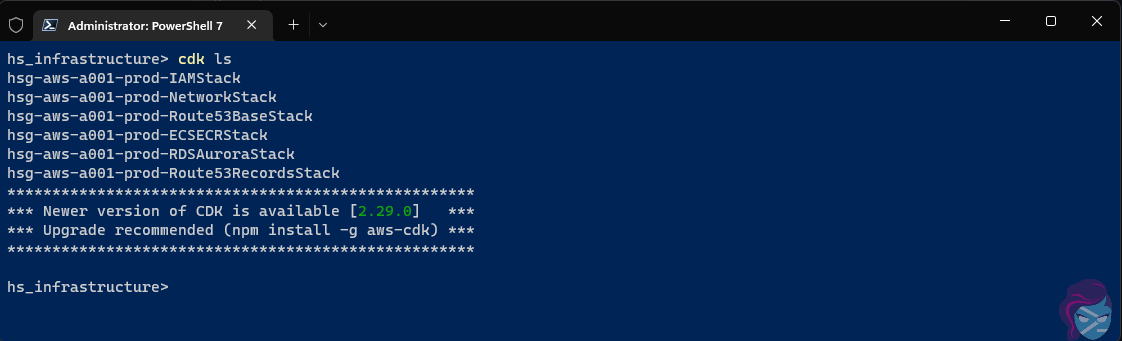
\includegraphics[width=1\linewidth]{cdk_ls.png}
    \caption{Proposed solution AWS stacks.}
    \label{fig:aws-stacks}
    \source{Own work.}
\end{figure}

Each of the stacks defines several services needed to build the whole overall infrastructure.
\begin{itemize}
    \item hsg-aws-a001-prod-IAMStack: Creates IAM user needed by the AWS elastic container service (ECS) and elastic container registry (ECR).
    \item hsg-aws-a001-prod-NetworkStack: Sets up the overall AWS infrastructure networking. Subnets, firewall rules, \textit{et cetera}. This is the longest stack in terms of lines of code, because it is made up of approximately 480 lines of code.
    \item hsg-aws-a001-prod-Route53BaseStack: This creates a hosted zone for the domain helloskygroup.com as well as a wildcard SSL certificate for the domain.
    \item hsg-aws-a001-prod-ECSECRStack: This spins up docker containers hosting the web application in the AWS ECS Fargate service. Fargate was used since it is a serverless service. A serverless service is a service that offloads the responsibility from developers to managed the actual physical servers hosting the deployed resources.
    \item hsg-aws-a001-prod-RDSAuroraStack: This deploys a MySQL database in the AWS relational database service (RDS).
    \item hsg-aws-a001-prod-Route53RecordsStack: This adds DNS records in the hosted zone created in the 'hsg-aws-a001-prod-Route53BaseStack' stack.
\end{itemize}

Once each stack is developed, the next step is to deploy it to AWS. Snippet \ref{code:hs_infrastructure_app_snippet_1} shows the \mintinline[breaklines, breakanywhere]{python}{main.py} code that basically imports all the created tasks in the AWS app and executes them. From there, the command \mintinline[breaklines, breakanywhere]{bash}{cdk deploy -all} needs to be executed from the root directory to deploy the resources and stacks defined in the app. Figure \ref{fig:aws-cdk-app-lifecycle} shows the full lifecycle of an AWS CDK app.

\begin{figure}[H]
    \centering 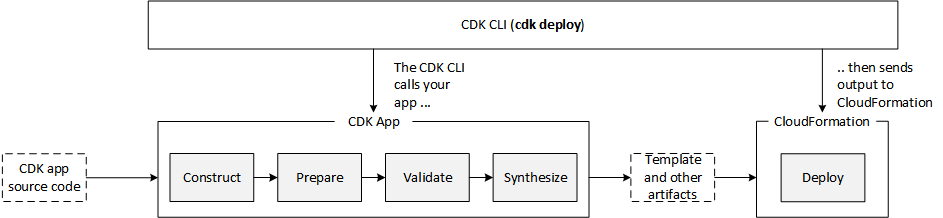
\includegraphics[width=1\linewidth]{aws_cdk_app_lifecycle.png}
    \caption{AWS CDK app lifecycle.}
    \label{fig:aws-cdk-app-lifecycle}
    \source{AWS documentation\cite{awscdkdocumentationapps}.}
\end{figure}

\begin{center}
    \captionsetup{type=listing}
    \inputminted[
        frame=single,
        framesep=2mm,
        baselinestretch=1.2,
        fontsize=\footnotesize,
        breaklines,
        breakanywhere,
        linenos
    ]{python}{config/code/47c895ea0838ad6366c2b0e53bb8c331/hs_infrastructure_app_snippet_1.py}
    \captionof{listing}{AWS CDK app.py snippet.}
    \label{code:hs_infrastructure_app_snippet_1}
\end{center}

%/--------------------------------- SECTION END ---------------------------------/%


%/-------------------------------- SECTION START --------------------------------/%

\section{AWS network and security configuration}
\label{sec:aws-network}

One of the challenges with implementing a networked system, especially on cloud platforms like AWS, is ensuring that traffic flows in the expected way with proper security in place. The proposed solution, being a networked solution involving communications to and from various applications, has a rigorous network design. Figure \ref{fig:aws-network-hld} shows how network within the proposed AWS infrastructure was designed.

AWS' Virtual Private Cloud also known as VPC concept, which is simply an isolated private network on the cloud. The VPC in the proposed solution is configured with network range 10.0.0.0/16 which is broken down in 3 subnets for each of the two availability zones that make the eu-central-1 (Frankfurt) region in which the AWS resources are deployed in.


%/------------------------------ SUB-SECTION START ------------------------------/%

\subsubsection*{Eu-central-1a availability zone}
\label{eu-central-1a-az}

\begin{itemize}
    \item Public subnet. Configured with network range 10.0.0.0/24.
    \item Private subnet. Configured with network range 10.0.2.0/24.
    \item Private-isolated subnet. Configured with network range 10.0.4.0/28.
\end{itemize}

%/------------------------------- SUB-SECTION END -------------------------------/%


%/------------------------------ SUB-SECTION START ------------------------------/%

\subsubsection*{Eu-central-1b availability zone}
\label{eu-central-1b-az}

\begin{itemize}
    \item Public subnet. Configured with network range 10.0.1.0/24.
    \item Private subnet. Configured with network range 10.0.3.0/24.
    \item Private-isolated subnet. Configured with network range 10.0.4.16/28.
\end{itemize}

\begin{figure}[H]
    \centering 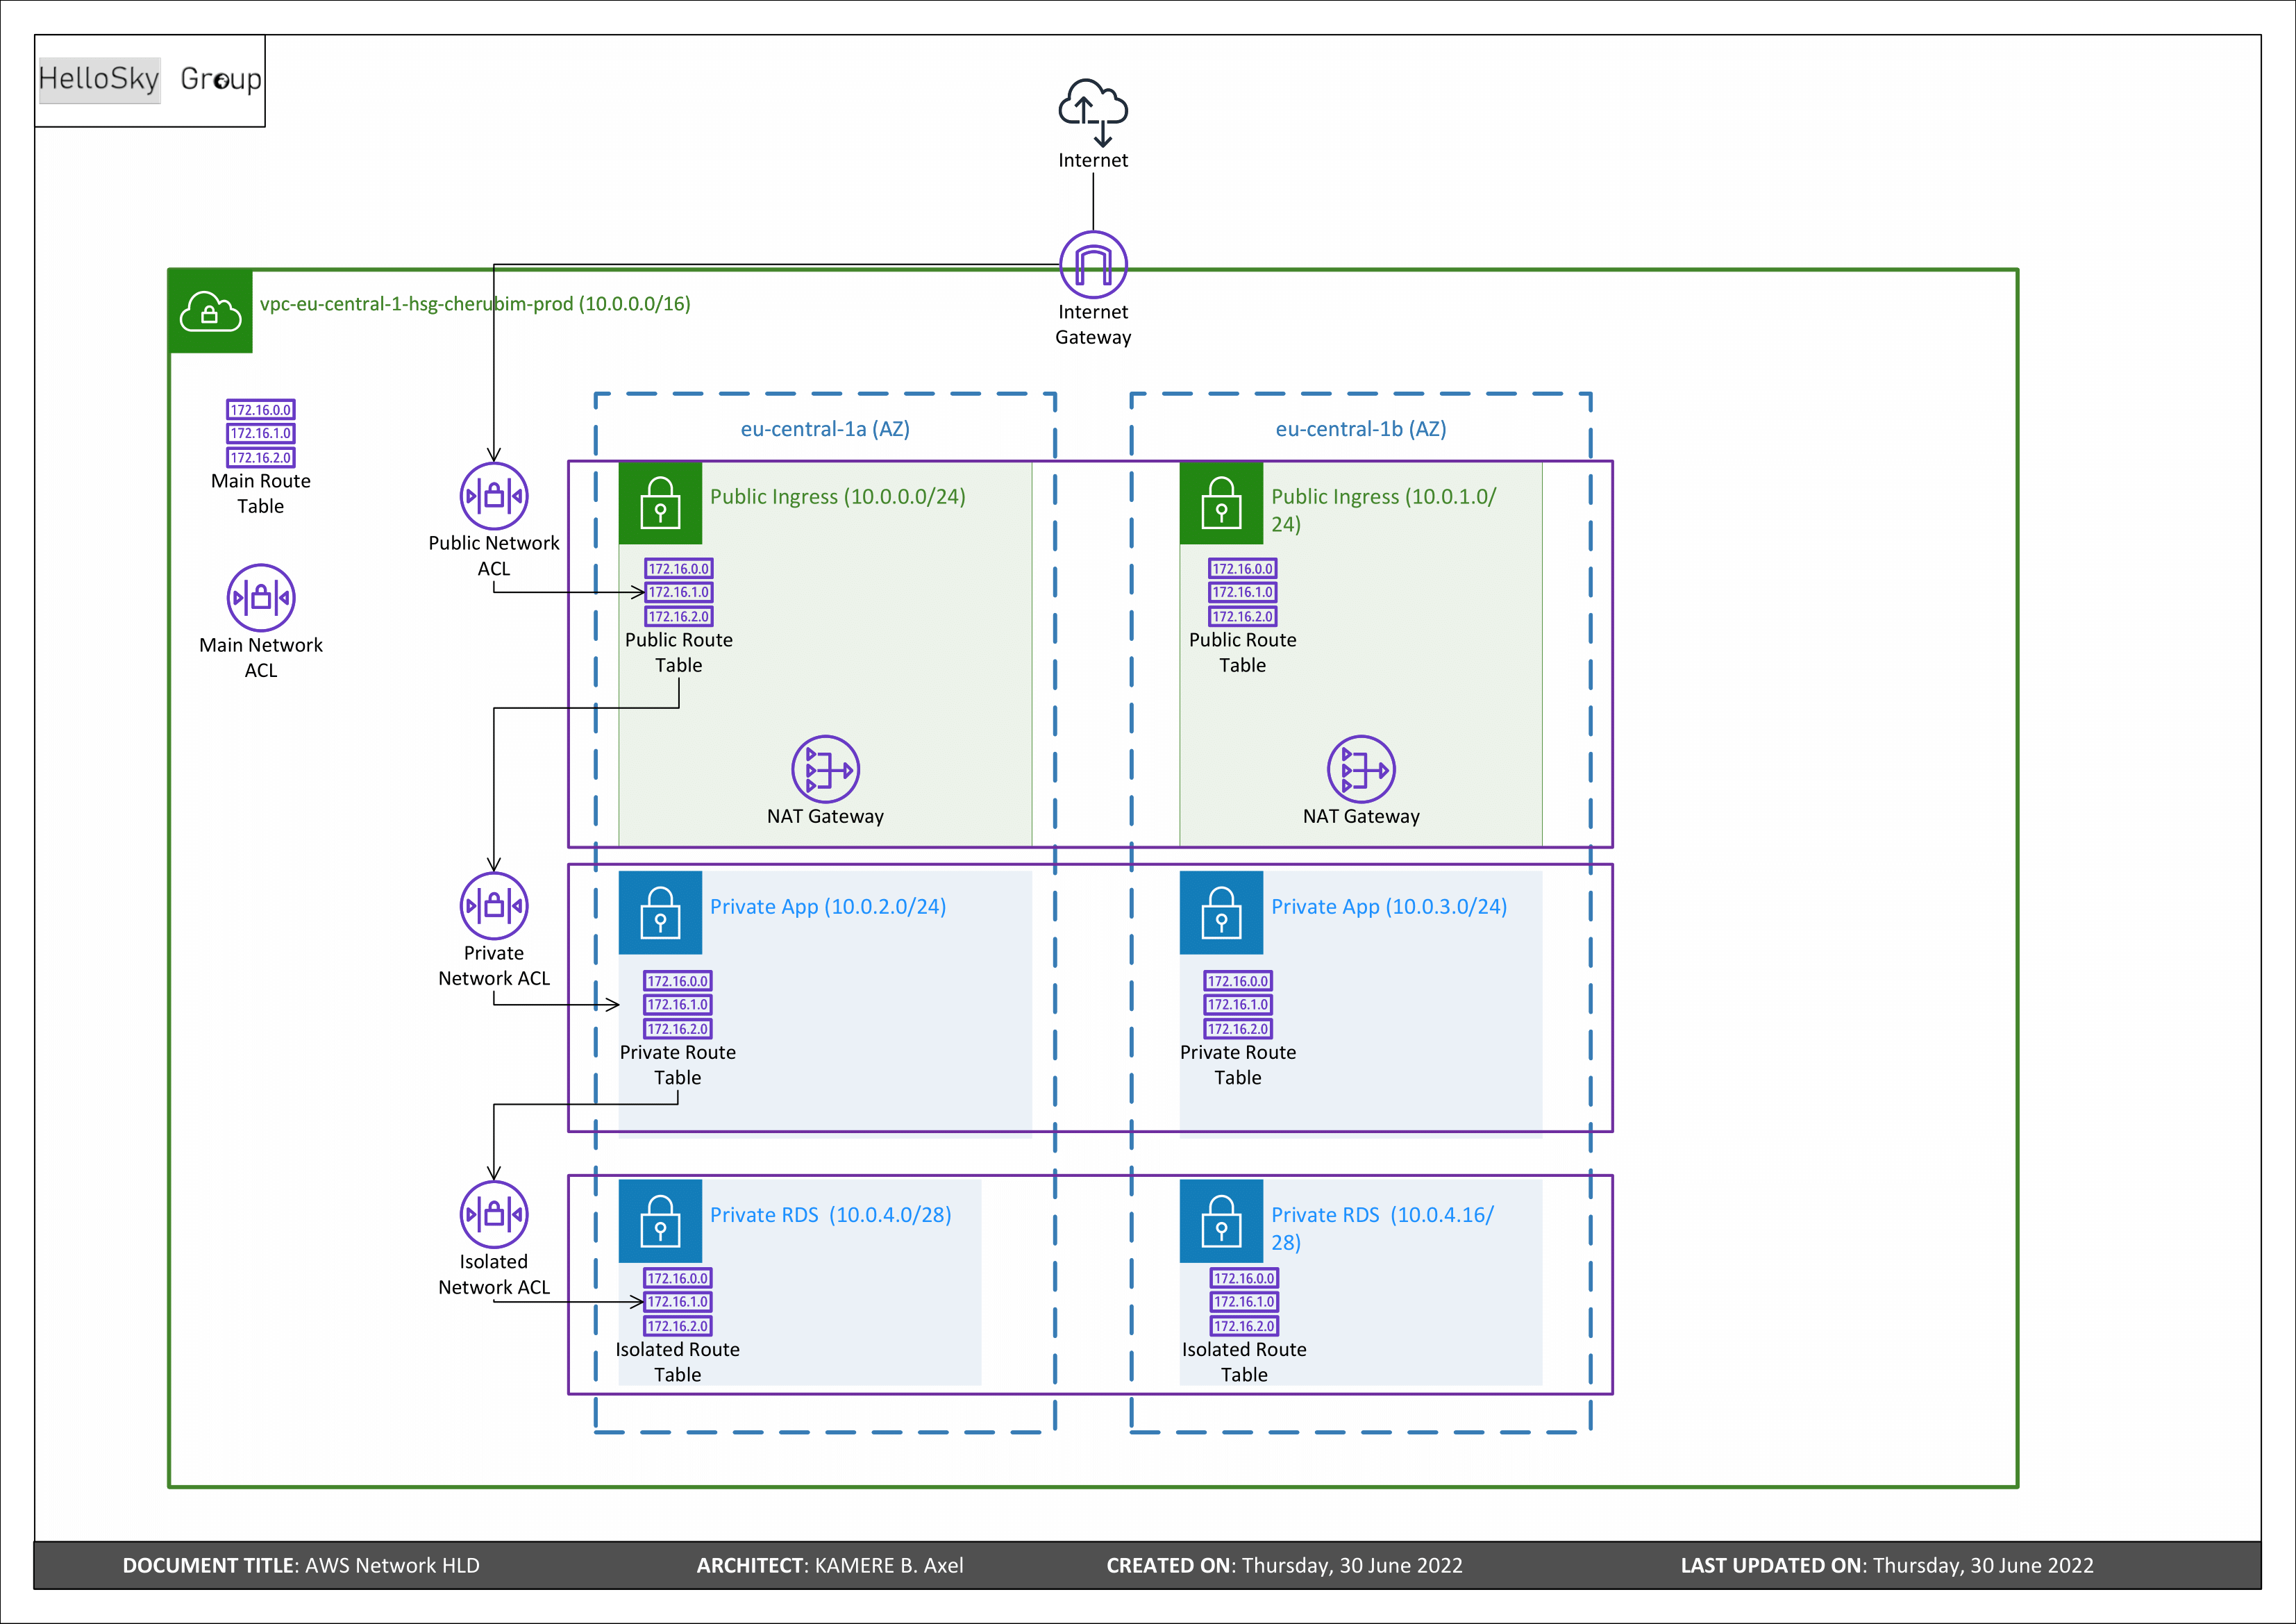
\includegraphics[width=1\linewidth]{aws_network_hld.png}
    \caption{AWS network high-level design.}
    \label{fig:aws-network-hld}
    \source{Own work. Designed with Microsoft Visio. Refer to \ref{subsec:ms-visio}.}
\end{figure}

%/------------------------------- SUB-SECTION END -------------------------------/%


%/------------------------------ SUB-SECTION START ------------------------------/%

\subsection{Public subnet}
\label{public-subnet}

The public subnet in this proposed solution does not contain any resources, except a Network Address Translation or NAT gateway that is used by resources in the private subnet to access the internet. Table \ref{table:public-subnet-inbound} and \ref{table:public-subnet-outbound} show the inbound and outbound traffic rules respectively configured on the public subnet network access control list or NACL.

\begin{table}[H]
    \centering
    \begin{tabular}{|c|c|c|c|c|c|}
        \hline
        \multicolumn{6}{|c|}{Inbound traffic}                               \\
        \hline
        Rule & Type        & Protocol & Port range & Source    & Allow/Deny \\
        \hline
        100  & HTTP (80)   & TCP (6)  & 80         & 0.0.0.0/0 & Allow      \\
        \hline
        110  & HTTPS (443) & TCP (6)  & 443        & 0.0.0.0/0 & Allow      \\
        \hline
        120  & Custom TCP  & TCP (6)  & 1024-65535 & 0.0.0.0/0 & Allow      \\
        \hline
        *    & All IPV4    & All      & All        & 0.0.0.0/0 & Deny       \\
        \hline
    \end{tabular}
    \caption{Public subnet NACL inbound traffic rules}
    \label{table:public-subnet-inbound}
\end{table}

\begin{itemize}
    \item \textbf{Rule 100:} Allows inbound HTTP traffic on port 80 towards any IPv4 address on the internet.
    \item \textbf{Rule 110:} Allows inbound HTTPS traffic on port 443 towards any IPv4 address on the internet.
    \item \textbf{Rule 120:} Allows returning TCP traffic from the internet responding to requests from the subnet. The specified port ranges are ephemeral ports as defined by the Internet Assigned Number Authority or IANA and Internet Engineering Task Force or IETF in their Request for Comments or RFC 6056 document \cite{rfc6056}.
    \item \textbf{Rule *:} Block every other non previously evaluated IPv4 traffic.
\end{itemize}

\begin{table}[H]
    \centering
    \begin{tabular}{|c|c|c|c|c|c|}
        \hline
        \multicolumn{6}{|c|}{Outbound traffic}                                \\
        \hline
        Rule & Type        & Protocol & Port range & Destination & Allow/Deny \\
        \hline
        100  & HTTP (80)   & TCP (6)  & 80         & 0.0.0.0/0   & Allow      \\
        \hline
        110  & HTTPS (443) & TCP (6)  & 443        & 0.0.0.0/0   & Allow      \\
        \hline
        120  & Custom TCP  & TCP (6)  & 1024-65535 & 0.0.0.0/0   & Allow      \\
        \hline
        *    & All IPV4    & All      & All        & 0.0.0.0/0   & Deny       \\
        \hline
    \end{tabular}
    \caption{Public subnet NACL outbound traffic rules}
    \label{table:public-subnet-outbound}
\end{table}

The rules' explanation are similar to those for inbound traffic in table \ref{table:public-subnet-inbound}, except that instead of inbound it is outbound.

%/------------------------------- SUB-SECTION END -------------------------------/%


%/------------------------------ SUB-SECTION START ------------------------------/%

\subsection{Private subnet}
\label{private-subnet}

Most of the infrastructure components are deployed in the private subnet where only specific traffic from the public and isolated-private subnets are allowed in. In this subnet is where the UAV command and control centre user interface is deployed, in containers using the AWS Fargate serverless service. The rules for this subnet have to be carefully defined so that;

\begin{itemize}
    \item Fargate services can pull docker images from docker hub public repositories on the internet.
    \item The UAV and several command and control application services can talk to each other.
\end{itemize}

Table \ref{table:private-subnet-inbound} and \ref{table:private-subnet-outbound} show the inbound and outbound traffic rules respectively configured on the private subnet network access control list or NACL.

\begin{table}[H]
    \centering
    \begin{tabular}{|c|c|c|c|c|c|}
        \hline
        \multicolumn{6}{|c|}{Inbound traffic}                                 \\
        \hline
        Rule & Type        & Protocol & Port range & Source      & Allow/Deny \\
        \hline
        100  & HTTP (80)   & TCP (6)  & 80         & 0.0.0.0/0   & Allow      \\
        \hline
        110  & HTTPS (443) & TCP (6)  & 443        & 0.0.0.0/0   & Allow      \\
        \hline
        120  & Custom TCP  & TCP (6)  & 1024-65535 & 0.0.0.0/0   & Allow      \\
        \hline
        130  & Custom TCP  & TCP (6)  & 3306       & 10.0.4.0/28 & Allow      \\
        \hline
        140  & Custom TCP  & TCP (6)  & 3306       & 10.0.5.0/28 & Allow      \\
        \hline
        *    & All IPV4    & All      & All        & 0.0.0.0/0   & Deny       \\
        \hline
    \end{tabular}
    \caption{Private subnet NACL inbound traffic rules}
    \label{table:private-subnet-inbound}
\end{table}

\begin{itemize}
    \item \textbf{Rule 100:} Allows inbound HTTP traffic on port 80. This is so that the AWS Elastic Container Service or ECS tasks can pull images from the public Docker Hub registry.
    \item \textbf{Rule 110:} Allows inbound HTTPS traffic on port 443.
    \item \textbf{Rule 120:} Allows returning TCP traffic from the internet responding to requests from the subnet.
    \item \textbf{Rule 130 and Rule 140:} Allows inbound traffic on port 3306 from MySQL database running in the AWS Relational Database Service or AWS within the isolated-private subnets of both the Availability Zones.
    \item \textbf{Rule *:} Blocks every other non previously evaluated IPv4 traffic.
\end{itemize}

\begin{table}[H]
    \centering
    \begin{tabular}{|c|c|c|c|c|c|}
        \hline
        \multicolumn{6}{|c|}{Outbound traffic}                                \\
        \hline
        Rule & Type        & Protocol & Port range & Destination & Allow/Deny \\
        \hline
        100  & HTTP (80)   & TCP (6)  & 80         & 0.0.0.0/0   & Allow      \\
        \hline
        110  & HTTPS (443) & TCP (6)  & 443        & 0.0.0.0/0   & Allow      \\
        \hline
        120  & Custom TCP  & TCP (6)  & 1024-65535 & 0.0.0.0/0   & Allow      \\
        \hline
        130  & Custom TCP  & TCP (6)  & 3306       & 10.0.4.0/28 & Allow      \\
        \hline
        140  & Custom TCP  & TCP (6)  & 3306       & 10.0.5.0/28 & Allow      \\
        \hline
        *    & All IPV4    & All      & All        & 0.0.0.0/0   & Deny       \\
        \hline
    \end{tabular}
    \caption{Private subnet NACL outbound traffic rules}
    \label{table:private-subnet-outbound}
\end{table}

\begin{itemize}
    \item \textbf{Rule 100:} Allows outbound HTTP traffic on port 80 towards any IPv4 address.
    \item \textbf{Rule 110:} Allows outbound HTTPS traffic on port 443 towards any IPv4 address.
    \item \textbf{Rule 120:} Allows all outbound response TCP traffic.
    \item \textbf{Rule *:} Blocks every other non previously evaluated IPv4 traffic.
\end{itemize}

%/------------------------------- SUB-SECTION END -------------------------------/%


%/------------------------------ SUB-SECTION START ------------------------------/%

\subsection{Isolated-private subnet}
\label{isolated-private-subnet}

The isolated-private subnet hosts the MySQL database running in AWS RDS. This subnet only talks to the private subnet, and has no direct connection to the internet. This improves the infrastructure security through not exposing the database instances directly to the internet.

<To-do: ADD NETWORK FLOW DESIGNS>

Describe the solution on a higher level. Discuss HLDs.

%/--------------------------------- SECTION END ---------------------------------/%


%/-------------------------------- SECTION START --------------------------------/%

\section{Software in the loop UAV simulator}
\label{sec:software-in-the-loop}

Software-in-the-loop or SITL is a technique used in prototyping where a robot's code or firmware is simulated and validated through software rather than on actual hardware. When hardware is involved in the simulation, it is called hardware-in-the-loop. This technique was used in the development of the proposed solution in this thesis due to its simplicity to set up compared to using actual hardware, which was the initial plan of the project and still is the long term plan of the project.

There are various ways in which software-in-the-loop can be implemented. This can involve using various simulators like Gazebo, Microsoft Airsim, \textit{et cetera}.

In this project, the simulator of choice was Gazebo <To-do: Cite gazebo>. Gazebo was deployed on a docker container running in headless mode \textit{id est} without the full Gazebo user interface but with only the console terminal. The simulator hosted PX4 autopilot for simulation. PX4 autopilot would then talk to a ground control station like QGroundControl via MAVLink to send and receive commands. The ground control station can also accept joystick connection with controllers like the Sony DualShock 4 wireless controller.

The proposed setup goes like this:

\begin{itemize}
    \item A Docker container running Gazebo headless and PX4 is spun up in headless mode. The container exposes a couple of ports; one for an off-board application to control the simulated drone via MAVLink API (UDP port 14551) as well as interfaces that can be used by a ground control station (UDP port 14550). The Docker image used is available on Docker Hub <To-do: Cite the source>. The command to run the container is:

          \mint[fontsize=\footnotesize, framesep=2mm, baselinestretch=1.2, breaklines, breakanywhere]{bash}|docker run --rm -it --env PX4_HOME_LAT=53.12758 --env PX4_HOME_LON=17.99353 jonasvautherin/px4-gazebo-headless:1.12.3|

          The container is given two environment variables that are used to set the home position of the simulated drone which in this case is the location of the WSG university.
    \item Once the container is running, a console will be presented where one can type in commands to control the drone. See figure <To-do: refer to an image of PX4 command after running the container.>
    \item With the container running, a GCS like QGroundControl can be connected to PX4 via UDP port 14550. From there, the drone's operation performance indicators can be visualized. See figure <To-do: refer to an image of the QGC>
    \item Also with the exposed off-board API port 14551, a custom application can be built to control the drone using programming languages like Python through the MAVSDK library. See figure <To-do: refer to an image of the Python MAVSDK code.>
\end{itemize}

Figure \ref{fig:sitl-hld} shows the high-level design of the proposed SITL setup described above.

\begin{figure}[H]
    \centering 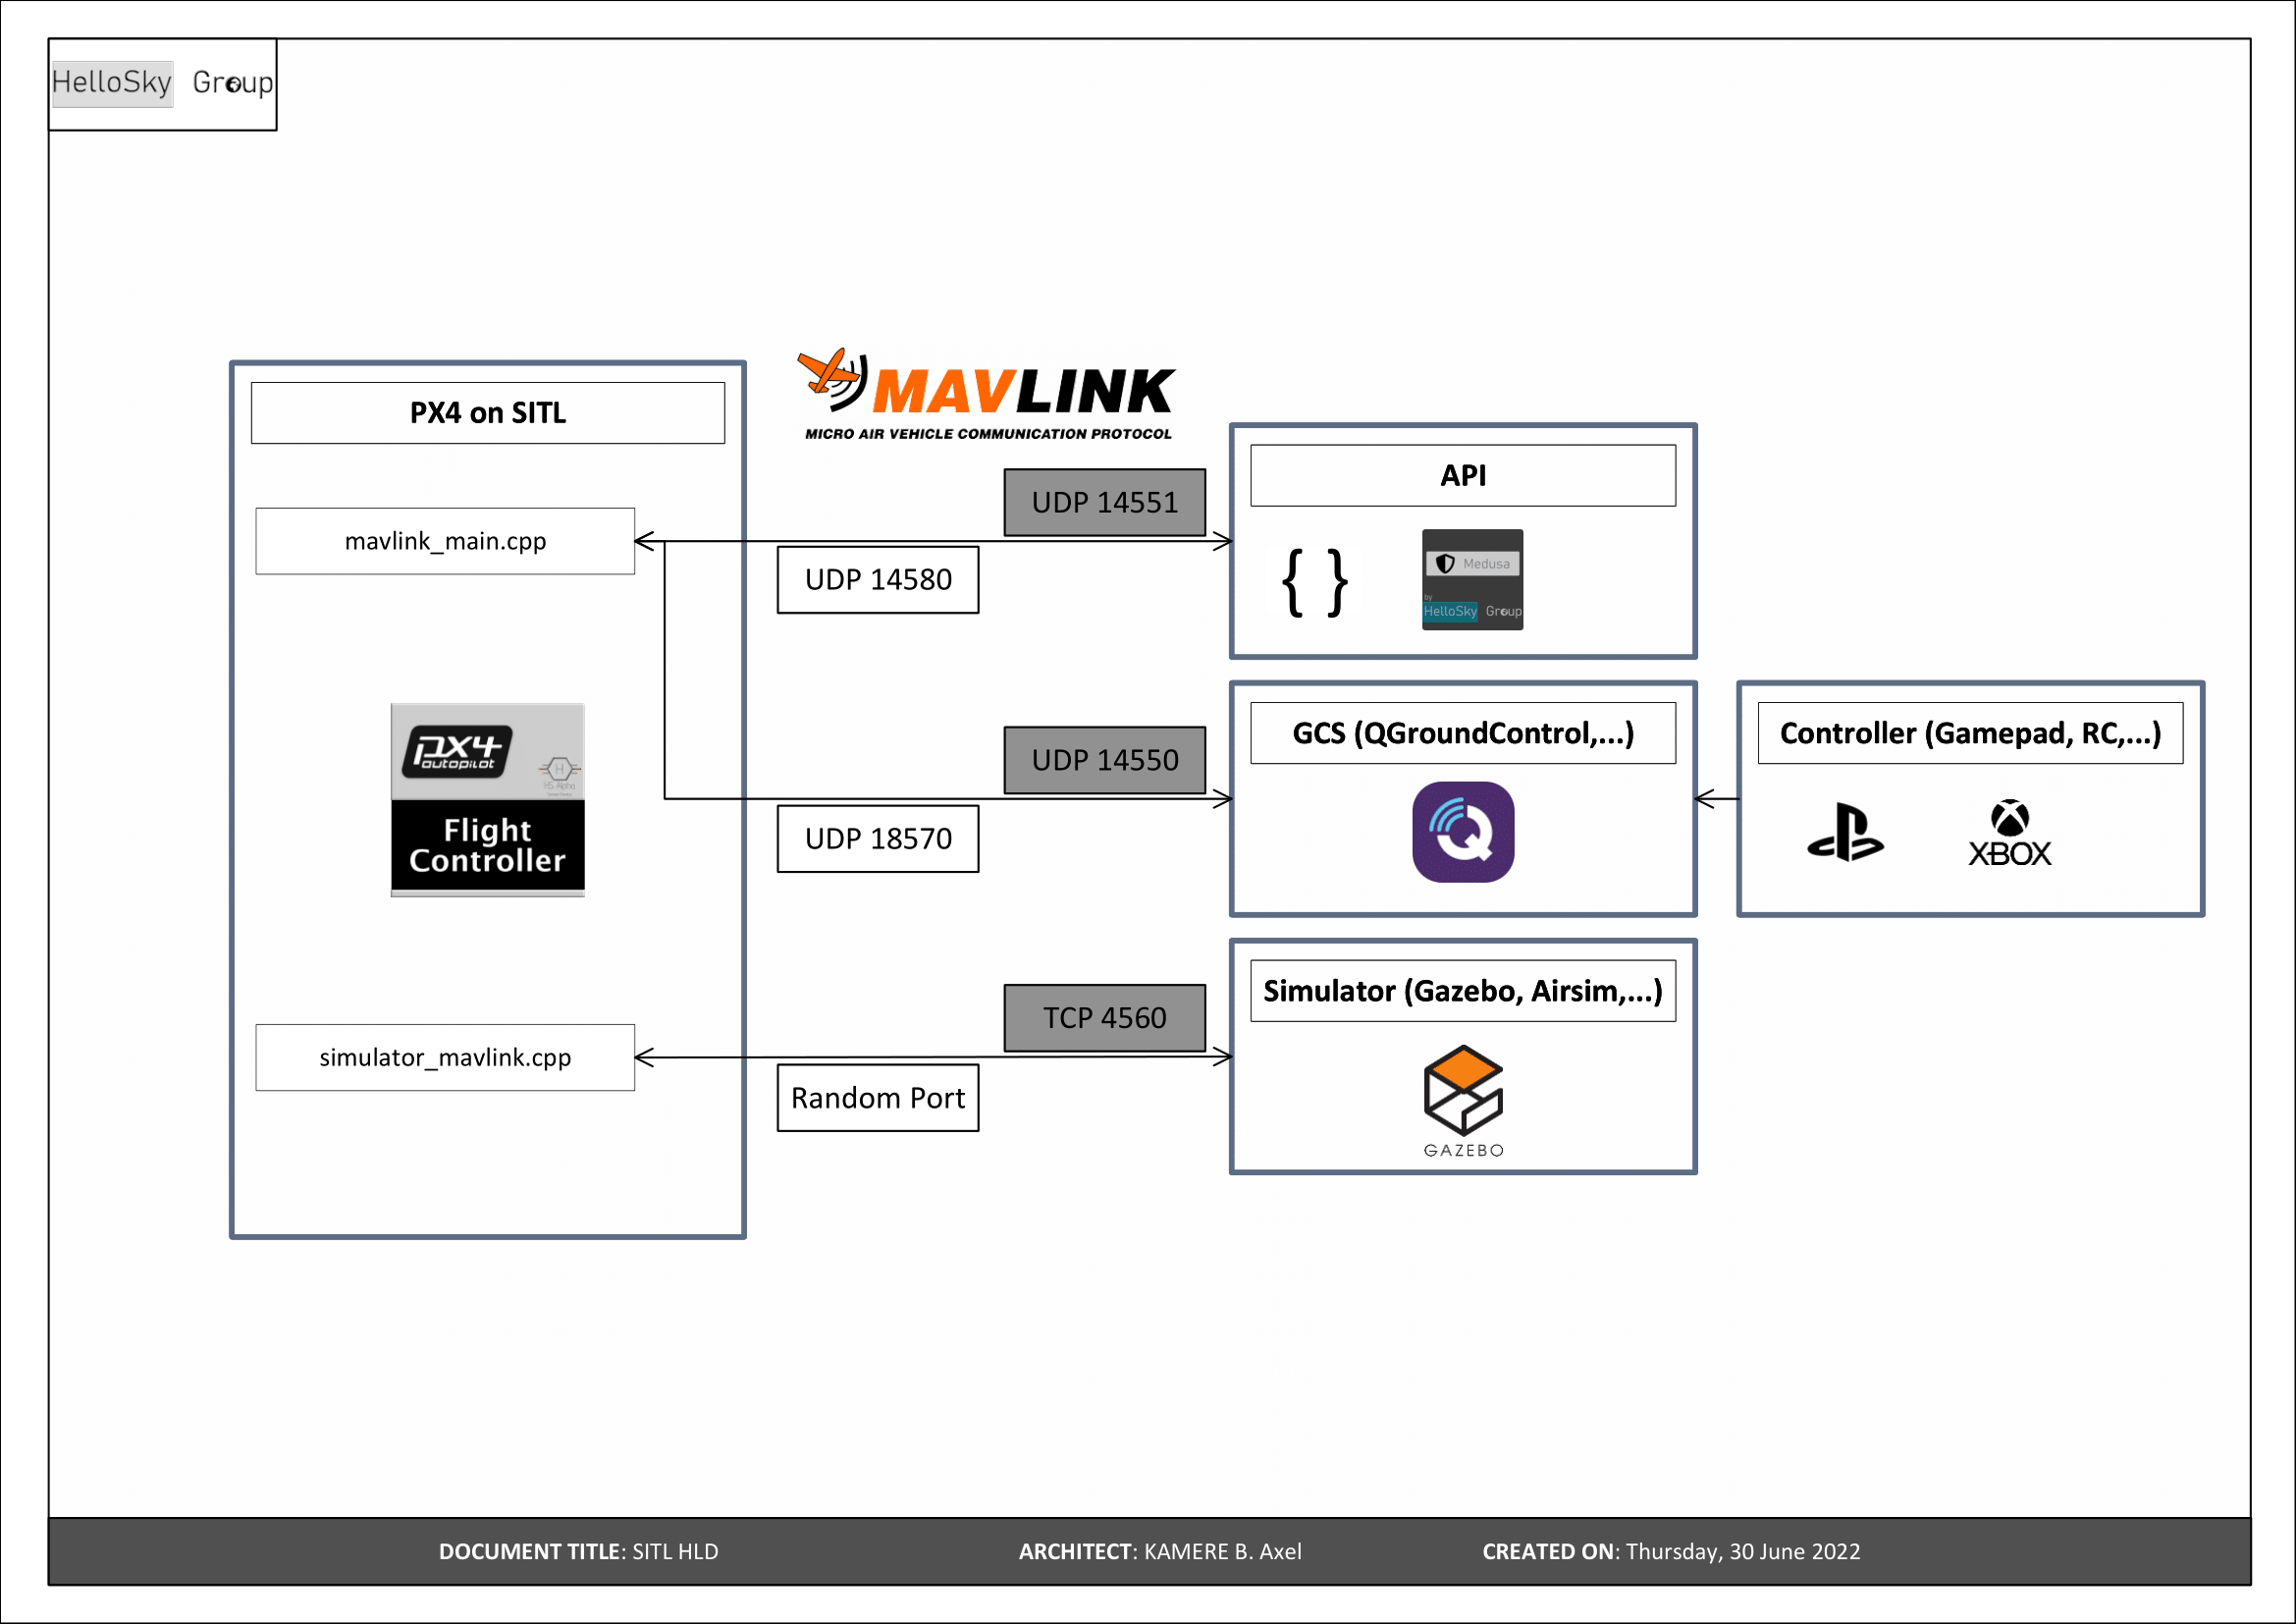
\includegraphics[width=1\linewidth]{sitl_hld.png}
    \caption{Proposed Simulation-In-The-Loop (SITL) architecture high-level design.}
    \label{fig:sitl-hld}
    \source{Own work. Designed with Microsoft Visio. Refer to \ref{subsec:ms-visio}.}
\end{figure}

%/--------------------------------- SECTION END ---------------------------------/%


%/-------------------------------- SECTION START --------------------------------/%

\section{UAV Communication}
<To-do: Talk about MAVLink... and how MAVLink is used in the project>

%/--------------------------------- SECTION END ---------------------------------/%

%/--------------------------------- CHAPTER END ---------------------------------/%


%/----------------------------- NOMENCLATURE START ------------------------------/%

\nomenclature[z-AZ]{AZ}{Availability Zone}
\nomenclature[z-NAT]{NAT}{Network Address Translation}
\nomenclature[z-VPC]{VPC}{Virtual Private Cloud}
\nomenclature[z-HTTP]{HTTP}{Hypertext Transfer Protocol}
\nomenclature[z-HTTPS]{HTTPS}{Hypertext Transfer Protocol Secured}
\nomenclature[z-ECS]{ECS}{Elastic Container Service}
\nomenclature[z-NACL]{NACL}{Network Access Control List}
\nomenclature[z-EC2]{EC2}{Elastic Cloud Compute}
\nomenclature[z-TCP]{TCP}{Transmisison Control Protocol}
\nomenclature[z-RDS]{RDS}{Relational Database Service}
\nomenclature[z-ALB]{ALB}{Application Load Balancer}
\nomenclature[z-RDS]{RDS}{Relational Database Service}
\nomenclature[z-IANA]{IANA}{Internet Assigned Number Authority}
\nomenclature[z-IETF]{IETF}{Internet Engineering Task Force}
\nomenclature[z-RFC]{RFC}{Request for Comments}
\nomenclature[z-PCB]{PCB}{Printed Circuit Board}
\nomenclature[z-SD]{SD (as in SD card)}{Secure Digital}
\nomenclature[z-GPS]{GPS}{Global Positioning System}
\nomenclature[z-S3]{S3 (as in AWS S3)}{Simple Storage Service}
\nomenclature[z-CLI]{CLI}{Command Line Interface}
\nomenclature[z-IAM]{IAM}{Identity Access Management}
\nomenclature[z-ECR]{ECR}{Elastic Container Registry}

%/------------------------------ NOMENCLATURE END -------------------------------/%
